\documentclass[lang=cn,a4paper,newtx,bibend=bibtex]{elegantpaper}
\usepackage{env}
\title{Problems of Chapter 10.5}
\author{张志心 \ 计科2106}
\date{\zhdate{2024/04/30}}
\usepackage{env}
\pgfplotsset{compat=1.17}
\addbibresource[location=local]{reference.bib}
\begin{document}
\maketitle

\begin{prob}[Exercise 10.156]
  Does the length of a short thick line segment in Figure 10.9 represent the one-step error in Definition
  10.159? If so, prove it; otherwise derive an expression of the
  represented quantity.
\end{prob}

\begin{solution}
  $\mathcal{L} \bm{u} (t_n) = \bm{u} (t_{n+1}) - \bm{u}(t_n) - k \Phi(\bm{u}(t_n), t_n; k)$,
  short thick line 的长度为
  \[
    \bm{u} (t_{n+1}) - \bm{u} (t_n) + \bm{U}^{n} - \bm{U}^{n+1} = 
    \bm{u} (t_{n+1}) - \bm{u} (t_n) - k \Phi (\bm{U}^n, t_n; k).
  \]
  所以不是 modified Euler 方法的单步误差,而是
  \[
    \mathcal{L} \bm{u} (t_n) + k(\Phi(\bm{u}(t_n), t_n; k) - \Phi (\bm{U}^n, t_n; k)).
  \]
\end{solution}

\begin{prob}[Exercise 10.158]
  Give a geometric interpretation of TR-BDF2 
  by drawing a figure similar to those for the improved
  Euler method and the modified Euler method.
\end{prob}

\begin{solution}~~\\
  \begin{figure}[H]
    \centering
    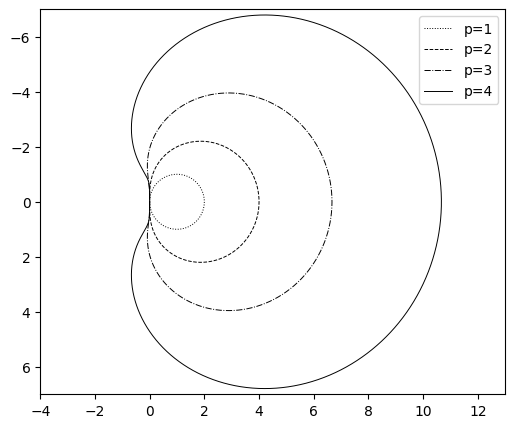
\includegraphics[width=0.6\textwidth]{4.png}
  \end{figure}
  以下几何解释中方程组的维数为$1$,即$(t,u)$是二维平面上的点。给定$t_n,U^n$的情况下,$U^{n+1}$将按如下步骤作出:
    \begin{enumerate}
        \item $P_1(t_n,U^n)$;
        \item $l_1$是过$P_1$的积分曲线在$t=t_n$处的切线,它的斜率为$f(U^n,t_n)$;
        \item $P_2$是$l_1$上横坐标为$t=t_n+\frac k4$的点,即$P_2(t_n+\frac k4,U^n+\frac k4 f(U^n,t_n))$;
        \item $l_2$:一条积分曲线在$t=t_n+\frac k2$的切线,该切线过$P_2$,它的斜率为$f(\cdot,t_n+\frac k2)$;
        \item $P_3$:$l_2$上横坐标为$t=t_n+\frac k2$的点,记其纵坐标为$U^*$,即$P_3(t_n+\frac k2,U^*)$;
        \item $P_4$:延长$P_1P_3$至横坐标为$t=t_n+\frac 23 k$,即$P_4(t_n+\frac 23 k,\frac 13(4U^*-U^n))$;
        \item $l_3$:一条积分曲线在$t=t_n+k$的切线,该切线过$P_4$,它的斜率为$f(\cdot,t_n+k)$;
        \item $P_5$:$l_3$上横坐标为$t=t_n+k$的点,记其纵坐标为$U^{n+1}$,即$P_5(t_n+k,\frac 13(4U^*-U^n+kf(U^{n+1},t_n+k)))$。
    \end{enumerate}
\end{solution}

\begin{prob}[Exercise 10.162]
  Use recursive Taylor expansions to derive
  the $k^3$ term in the one-step error $\mathcal{L}\bm{u} (t_n)$ 
  of the explicit midpoint method, 
  verifying $\mathcal{L}\bm{u} (t_n) = \Theta (k^3)$, 
  i.e., the explicit midpoint method is second-order accurate.
\end{prob}

\begin{proof}
\equ{ 
  \mathcal{L} \bm{u} (t_n) &= \bm{u}(t_{n+1}) - \bm{u}(t_n) - k \Phi (\bm{u}(t_n), t_n; k) \\
  &= (\bm{u}(t_n) + k \bm{u}'(t_n) + \frac{k^2}2 \bm{u}''(t_n) + \frac{k^3}6 \bm{u}'''(t_n) + O(k^4)) - \bm{u} (t_n) - k \bm{f}(\bm{u} (t_n) + \frac{k}2 \bm{f}(\bm{u}(t_n), t_n), t_n + \frac{k}2) \\
  &= k \bm{u}'(t_n) + \frac{k^2}2 \bm{u}''(t_n) + \frac{k^3}6 \bm{u}'''(t_n) - k \bm{f} (\bm{u}(t_n) + \frac{k}2 \bm{u}'(t_n), t_n + \frac{k}2) + O(k^4) \\
  &= k \bm{u}' (t_n)+ \frac{k^2}2 \bm{u}''(t_n) + \frac{k^3}6 \bm{u}'''(t_n) - k \bm{f} (\bm{u}(t_n), t_n) - \frac{k^2}2 \bm{f}_t (\bm{u}(t_n), t_n) - \frac{k^2}2 \bm{u}'(t_n) \bm{f}_n(\bm{u}(t_n), t_n) \\
  & \quad - \frac{k^3}8 \bm{f}_{tt}(\bm{u}(t_n), t_n) - \frac{k^3}{8} \bm{u}'(t_n)^2 \bm{f}_{uu} (\bm{u}(t_n), t_n) - \frac{k^3}4 \bm{u}'(t_n) \bm{f}_{ut} (\bm{u}(t_n), t_n)
}
因为
\equ{
  &\bm{u}' = \bm{f},\\
  &\bm{u}'' = \bm{f}_u \bm{u}' + \bm{f}_t = \bm{f}_u \bm{f} + \bm{f}_t, \\
  &\bm{u}''' = \bm{f}_{uu} \bm{f} \bm{u}' + \bm{f}_{ut} \bm{f} + \bm{f}_u^2 \bm{u}' + \bm{f}_u \bm{f}_t + \bm{f}_{ut} \bm{u}' + \bm{f}_{tt} = \bm{f}_{uu} \bm{f}^2 + 2 \bm{f}_{ut} \bm{f} + \bm{f}_u^2 \bm{f} + \bm{f}_u \bm{f}_t + \bm{f}_{tt}
}
所以
\equ{
  \mathcal{L} \bm{u} (t_n) &= k (\bm{u}' - \bm{f}) + \frac{k^2}2 (\bm{u}'' - \bm{f}_t - \bm{f}_u \bm{f}) + k^3 (\frac16 \bm{u}''' - \frac{\bm{f}_{tt} + 2 \bm{f}_{ut} \bm{f} + \bm{f}_{uu} \bm{f}^2}{8}) + O(k^4) \\
  &= k^3 (\frac{\bm{u}'''}6 - \frac{\bm{f}_{tt} + 2 \bm{f}_{ut} \bm{f} + \bm{f}_{uu} \bm{f}^2}{8}),
}
系数为
\equ{
  & \frac{\bm{u}'''(t_n)}{6} - \frac{\bm{f}_tt(\bm{u}(t_n), t_n) + 2 \bm{f}_{ut}(\bm{u}(t_n), t_n) \bm{f}(\bm{u}(t_n), t_n) + \bm{f}_{uu} (\bm{u}(t_n), t_n) \bm{f}(\bm{u}(t_n), t_n)^2}8.
}
即 $\mathcal{L} \bm{u} (t_n) = O(k^3)$,所以 explicit 中点法有二阶精度。
\end{proof}

\begin{prob}[Exercise 10.171]
  Show that the TR-BDF2 method in (10.106) satisfies
  \[
    R(z) = \dfrac{1 + \frac5{12}z}{1 - \frac7{12}z + \frac1{12}z^2},
  \]
  and $R(z) - e^z = O(z^3)$ as $z \to 0$.
\end{prob}

\begin{solution}
  对 IVP $\bm{u}' = \lambda \bm{u}$,有
  \[
    \Cases{
      \bm{U}^{*} = \bm{U}^n + \frac{k}4 (\lambda \bm{U}^n + \lambda \bm{U}^*) \\
      \bm{U}^{n+1} = \frac13 (4 \bm{U}^* - \bm{U}^n + k \lambda \bm{U}^{n+1})
    }
  \]
  $\bm{U}^* = \bm{U}^n + \frac{z}4 (\bm{U}^n + \bm{U}^*) \Rightarrow \bm{U}^* = \dfrac{1 + \frac{z}4}{1 - \frac{z}4} \bm{U}^n$.\\
  $\bm{U}^{n+1} = \dfrac{4 \bm{U}^* - \bm{U}^n + z\bm{U}^{n+1}}{3} \Rightarrow \bm{U}^{n+1} = \dfrac{4 \bm{U}^* - \bm{U}^n}{3 - z} = \dfrac{4\frac{(4 + z)}{4 - z} - 1}{3 - z} \bm{U}^n = \dfrac{5z + 12}{(z - 3)(z - 4)} = \dfrac{1 + \frac{5}{12}z}{1 - \frac{7}{12}z + \frac1{12}z^2}$.
  \equ{
    R(z) &= \frac{9}{1 - \frac{z}3} - \frac{8}{1 - \frac{z}4} \\
    &= 9(1 + \frac{z}3 + \frac{z^2}{9} + \frac{z^3}{27} + O(z^4)) - 8(1 + \frac{z}{4} + \frac{z^2}{16} + \frac{z^3}{64} + O(z^4)) \\
    &= 1 + z + \frac{z^2}2 + \frac{5 z^3}{24} + O(z^4) \\
    &= e^z + O(z^3).
  }
\end{solution}

\begin{prob}[Exercise 10.176]
  Reproduce the results in Example 10.175
and explain in your own language why the first-order backward
 Euler method is superior to the second-order trapezoidal method.
\end{prob}

\begin{solution}
  以下是Euler method求解以及画图的代码:该程序计算了不同步长和 $\eta$ 下的无穷范数。
\begin{verbatim}
function backward_euler
    solve(-1e6, 3, 0.2, 1);
    figure;
    t = (0:30)/10;
    Ans = exact(-1e6, 1, t);
    plot(t, Ans);
    hold on;
    plot(t, solve(-1e6, 3, 0.1, 1));
    
    solve(-1e6, 3, 0.05, 1);
    solve(-1e6, 3, 0.2, 1.5);
    t = (0:30)/10;
    Ans = exact(-1e6, 1.5, t);
    plot(t, Ans);
    hold on;
    plot(t, solve(-1e6, 3, 0.1, 1.5));
    
    solve(-1e6, 3, 0.05, 1.5);
end

function P = exact(lmd, u0, t)
    P = exp(lmd * t) .* (u0 - 1) + cos(t);
end

function P = step(lmd, k, u, t)
    t1 = t + k;
    P = (u - k * (lmd * cos(t1) + sin(t1))) / (1 - k * lmd);
end

function P = solve(lmd, T, k, u0)
    N = floor(T / k);
    u = zeros(1, N);
    u(1) = u0;
    err = 0;
    for i = 1:N
        u(i+1) = step(lmd, k, u(i), (i-1)*k);
        exact_value = exact(lmd, u0, i*k);
        err = max(err, abs(u(i+1) - exact_value));
    end
    fprintf("k = %f, u0 = %f, err = %e\n", k, u0, err);
    P = u;
end
\end{verbatim}
程序输出:
\begin{verbatim}
  >> backward_euler
  k = 0.200000, u0 = 1.000000, err = 9.900173e-08
  k = 0.100000, u0 = 1.000000, err = 4.987457e-08
  k = 0.050000, u0 = 1.000000, err = 2.498388e-08
  k = 0.200000, u0 = 1.500000, err = 2.400986e-06
  k = 0.100000, u0 = 1.500000, err = 4.950075e-06
  k = 0.050000, u0 = 1.500000, err = 9.974816e-06
\end{verbatim}
作图并与真解对比:发现曲线几乎重合,Backward-Euler对于本问题是稳定的。
\begin{figure}[H]
  \centering
  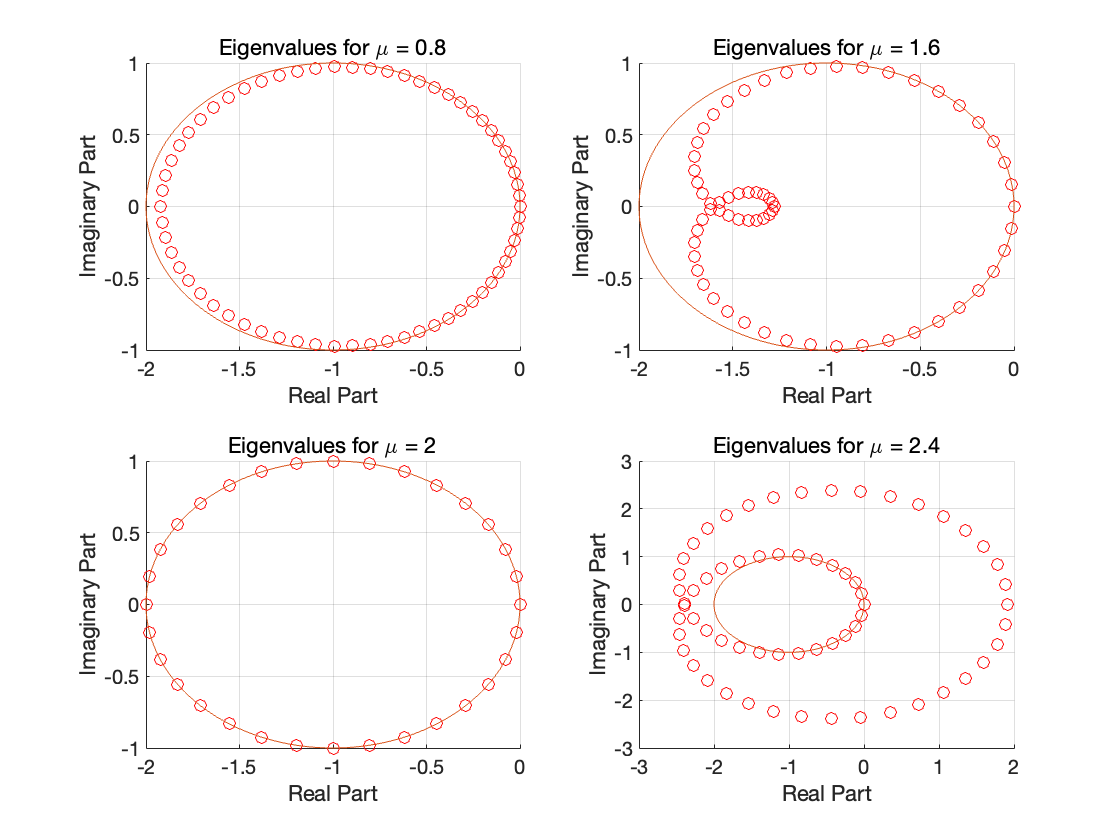
\includegraphics[width=0.5\textwidth]{1.png}
\end{figure}

对于 trapezoidal 方法,使用了不同的 step 函数,代码如下:
\begin{verbatim}
  function backward_euler
    solve(-1e6, 3, 0.2, 1);
    figure;
    t = (0:30)/10;
    Ans = exact(-1e6, 1, t);
    plot(t, Ans);
    hold on;
    plot(t, solve(-1e6, 3, 0.1, 1));
    
    solve(-1e6, 3, 0.05, 1);
    solve(-1e6, 3, 0.2, 1.5);
    t = (0:30)/10;
    Ans = exact(-1e6, 1.5, t);
    plot(t, Ans);
    hold on;
    plot(t, solve(-1e6, 3, 0.1, 1.5));
    
    solve(-1e6, 3, 0.05, 1.5);
end

function P = exact(lmd, u0, t)
    P = exp(lmd * t) .* (u0 - 1) + cos(t);
end

function P = step(lmd, k, u, t)
    t1 = t + k;
    P = (u - k * (lmd * cos(t1) + sin(t1))) / (1 - k * lmd);
end
\end{verbatim}
程序输出:
\begin{verbatim}
  >> trapezoidal
  k = 0.200000, u0 = 1.000000, err = 5.547095e-07
  k = 0.100000, u0 = 1.000000, err = 5.263548e-07
  k = 0.050000, u0 = 1.000000, err = 5.128314e-07
  k = 0.200000, u0 = 1.500000, err = 4.999898e-01
  k = 0.100000, u0 = 1.500000, err = 4.999799e-01
  k = 0.050000, u0 = 1.500000, err = 4.999600e-01
\end{verbatim}
对于 $\eta = 1$,求解误差很小,图像与真解几乎重合:
\begin{figure}[H]
  \centering
  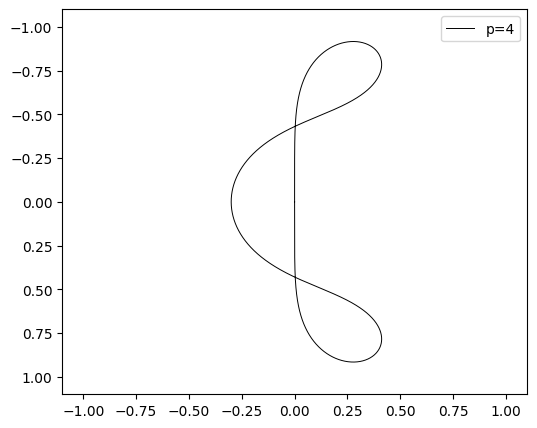
\includegraphics[width=0.5\textwidth]{2.png}
\end{figure}
但是对于 $\eta = 1.5$,求解结果在真实解附近来回振荡并不收敛:
\begin{figure}[H]
  \centering
  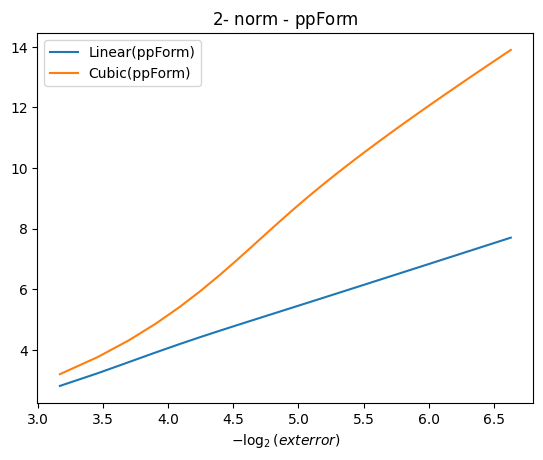
\includegraphics[width=0.5\textwidth]{3.png}
\end{figure}
Backward Euler方法是 L 稳定的,但是 trapezoidal 方法不是,因此前者在
求解特征值很大的问题时对于初值的敏感程度不会过大,收敛效果更好。
\end{solution}
\end{document}